\chapter{THIẾT KẾ SEQUENCE DIAGRAM CHO CÁC LUỒNG NGHIỆP VỤ CHÍNH}

\section{Thiết kế Sequence Diagram cho nghiệp vụ Nhập kho}

Sơ đồ tuần tự nghiệp vụ Nhập kho mô tả chi tiết thứ tự gửi và nhận thông điệp theo trục thời gian giữa Thủ kho, Giao diện React, Router Nhập kho (imports.py), SQLAlchemy Session và Cơ sở dữ liệu CSDL.

Khi thủ kho bấm 'Xác nhận nhập kho', hệ thống thực hiện mở Transaction, thêm bản ghi phiếu nhập, lặp qua danh sách sản phẩm để thêm chi tiết nhập, cập nhật cộng tồn kho vào bảng inventory và ghi bản ghi nhật ký biến động kho stock\_movements trước khi thực thi Commit.

Sơ đồ tuần tự nghiệp vụ Nhập kho được thể hiện tại Hình 7.1.

\begin{figure}[h!]
\centering
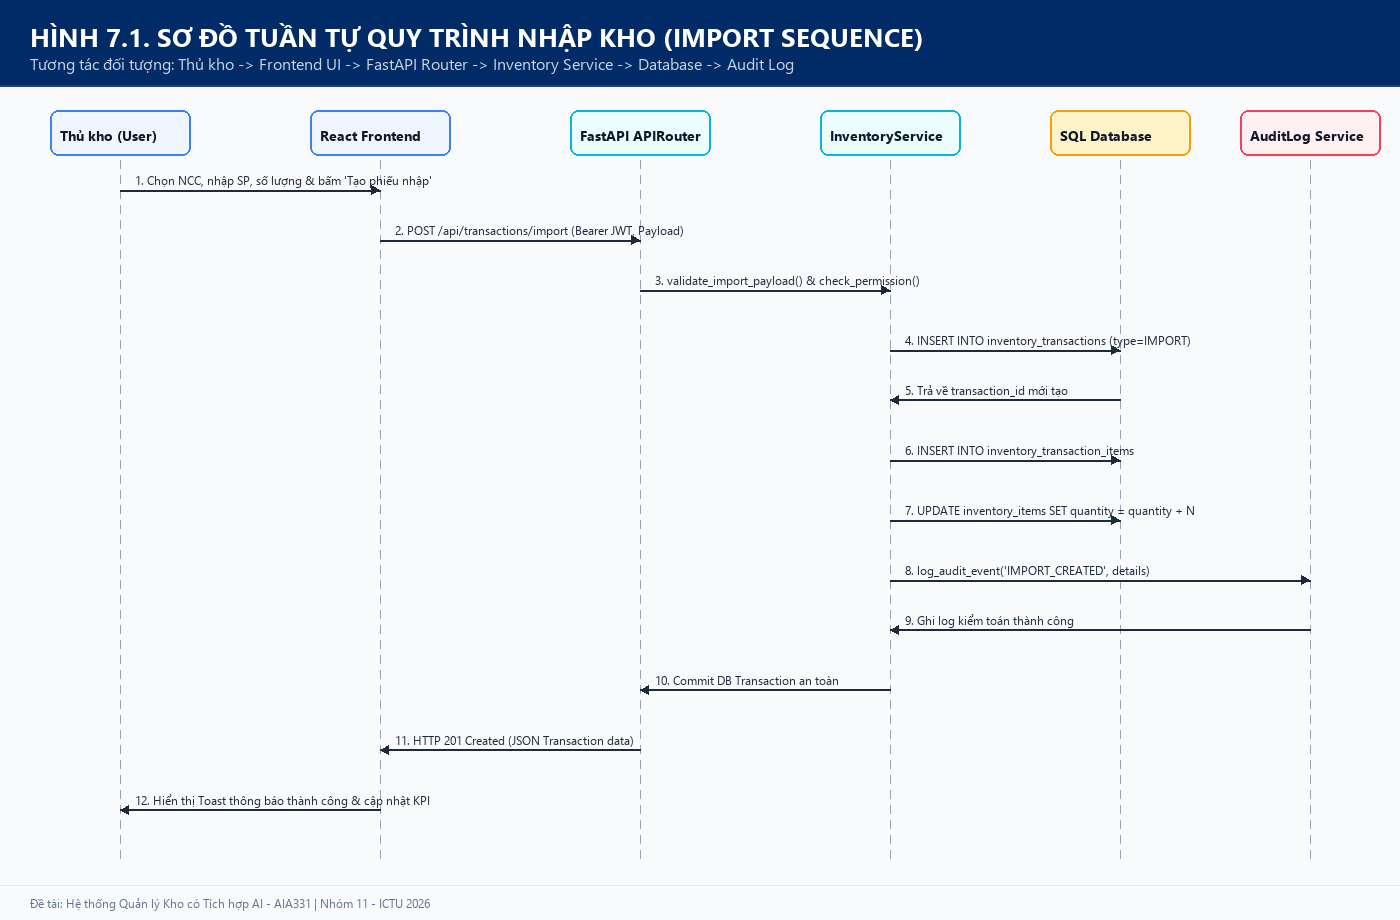
\includegraphics[width=0.92\textwidth]{figures/sequence_import.png}
\caption{Sơ đồ tuần tự (Sequence Diagram) nghiệp vụ Nhập kho và cập nhật tăng tồn}
\end{figure}

\section{Thiết kế Sequence Diagram cho nghiệp vụ Xuất kho và phòng ngừa xuất âm}

Sơ đồ tuần tự nghiệp vụ Xuất kho làm nổi bật cơ chế kiểm soát nghiêm ngặt nhằm ngăn chặn tuyệt đối tình trạng âm tồn kho:

1. Thủ kho gửi yêu cầu xuất kho kèm danh sách sản phẩm và số lượng.

2. Router exports.py gọi CSDL để khóa và đọc số lượng tồn kho khả dụng hiện tại của từng mặt hàng.

3. Nhánh rẽ Alt [Số lượng xuất > Tồn kho khả dụng]: Router kích hoạt Rollback, từ chối toàn bộ giao dịch, trả về HTTP 400 Bad Request kèm thông báo lỗi chi tiết cho người dùng.

4. Nhánh rẽ Alt [Số lượng xuất <= Tồn kho khả dụng]: Router trừ số lượng tồn, ghi nhận chi tiết phiếu xuất, tạo bản ghi biến động kho và thực thi Commit thành công.

Sơ đồ tuần tự nghiệp vụ Xuất kho được thể hiện tại Hình 7.2.

\begin{figure}[h!]
\centering
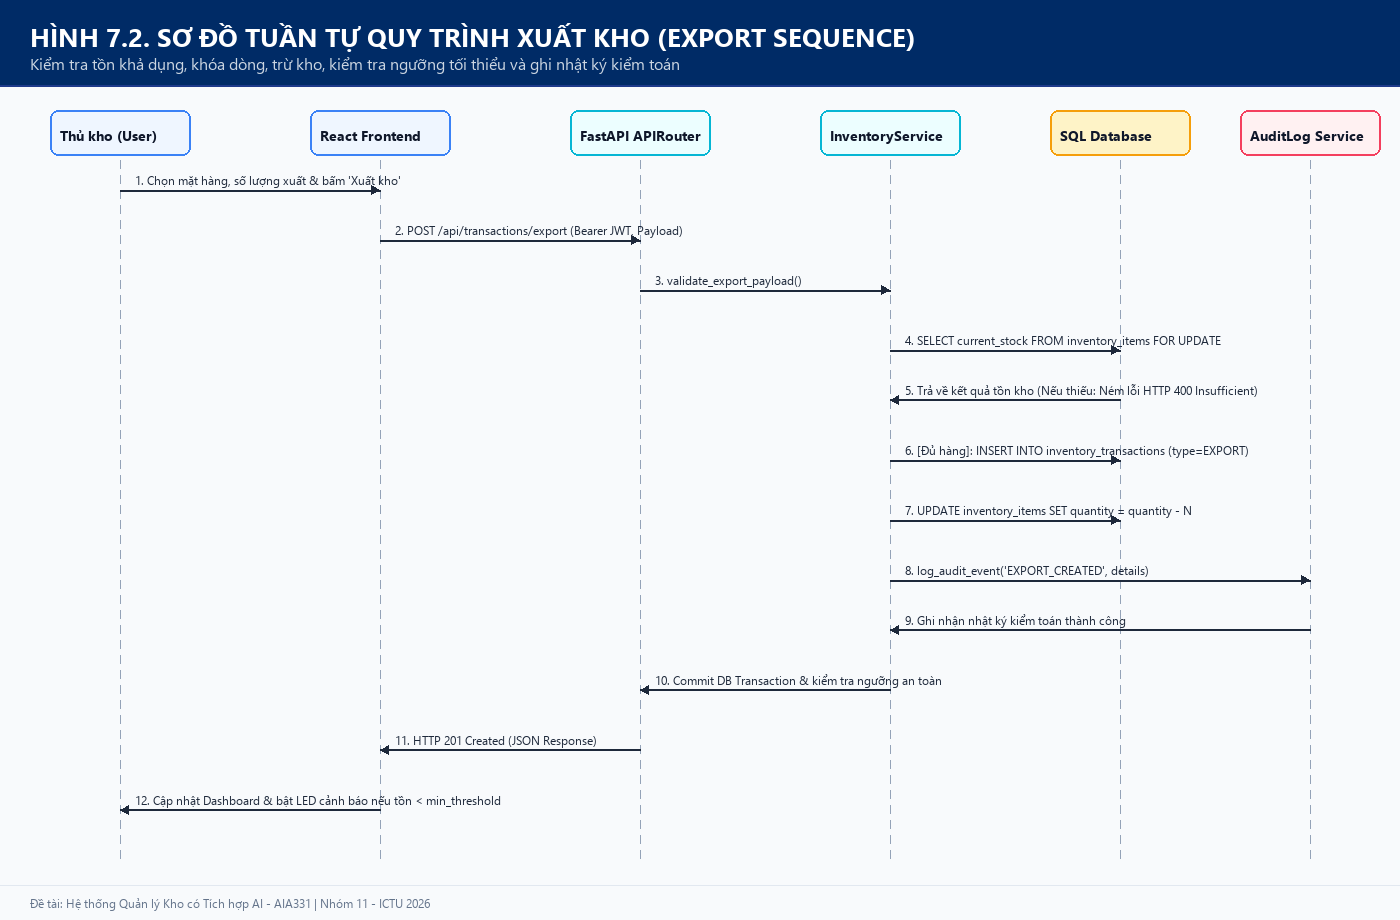
\includegraphics[width=0.92\textwidth]{figures/sequence_export.png}
\caption{Sơ đồ tuần tự (Sequence Diagram) nghiệp vụ Xuất kho có kiểm soát chống âm tồn}
\end{figure}

